\section{Auswertung}
\label{sec:Auswertung}


\subsection{Kennlinienschar}

In \autoref{tab:kennlinien} sind die Messdaten der fünf Kennlinien aufgetragen.
\begin{table}
  \centering
  \caption{Messwerte der fünf Kennlinien.}
  \label{tab:kennlinien}
  \begin{tabular}{c c c c c c}
    \toprule
    & \multicolumn{1}{c}{$I_{\text{Heiz}} = \qty{1.9}{\ampere}$} &
      \multicolumn{1}{c}{$I_{\text{Heiz}} = \qty{2.0}{\ampere}$} &
      \multicolumn{1}{c}{$I_{\text{Heiz}} = \qty{2.1}{\ampere}$} &
      \multicolumn{1}{c}{$I_{\text{Heiz}} = \qty{2.2}{\ampere}$} &
      \multicolumn{1}{c}{$I_{\text{Heiz}} = \qty{2.4}{\ampere}$} \\
      \cmidrule(lr){2-2}\cmidrule(lr){3-3}\cmidrule(lr){4-4}\cmidrule(lr){5-5}\cmidrule(lr){6-6}

    $U \mathbin{/} \unit{\volt}$ &
    $I \mathbin{/} \unit{\milli\ampere}$ &
    $I \mathbin{/} \unit{\milli\ampere}$ &
    $I \mathbin{/} \unit{\milli\ampere}$ & 
    $I \mathbin{/} \unit{\milli\ampere}$ &
    $I \mathbin{/} \unit{\milli\ampere}$ \\
    \midrule
    0   &  0,00 &    0,00 &    0,00 &   0,000 &    0,00 \\
    5   &  0,01 &    0,01 &    0,01 &   0,020 &    0,03 \\
    10  &  0,03 &    0,04 &    0,05 &   0,050 &    0,10 \\
    15  &  0,05 &    0,06 &    0,10 &   0,100 &    0,18 \\
    20  &  0,07 &    0,09 &    0,16 &   0,200 &    0,26 \\
    25  &  0,08 &    0,12 &    0,22 &   0,290 &    0,37 \\
    30  &  0,08 &    0,14 &    0,26 &   0,370 &    0,48 \\
    35  &  0,08 &    0,15 &    0,29 &   0,450 &    0,60 \\
    40  &  0,08 &    0,15 &    0,32 &   0,510 &    0,72 \\
    45  &  0,08 &    0,15 &    0,33 &   0,570 &    0,86 \\
    50  &  0,08 &    0,17 &    0,34 &   0,620 &    0,99 \\
    60  &       &         &    0,35 &   0,690 &    1,25 \\
    70  &       &         &    0,36 &   0,730 &    1,48 \\
    80  &       &         &         &   0,750 &    1,68 \\
    90  &       &         &         &   0,760 &    1,89 \\
    100 &       &         &         &   0,770 &    2,07 \\
    110 &       &         &         &   0,841 &    2,33 \\
    120 &       &         &         &   0,780 &    2,33 \\
    130 &       &         &         &         &    2,43 \\
    140 &       &         &         &         &    2,50 \\
  \bottomrule
  \end{tabular}
\end{table}

Zur Bestimmung des Sättigungstroms $I_{\text{S}}$ werden die Messdaten in \autoref{fig:k} graphisch dargestellt.
\begin{figure}
  \centering
  
  \begin{subfigure}{0.49\columnwidth}
  \centering
  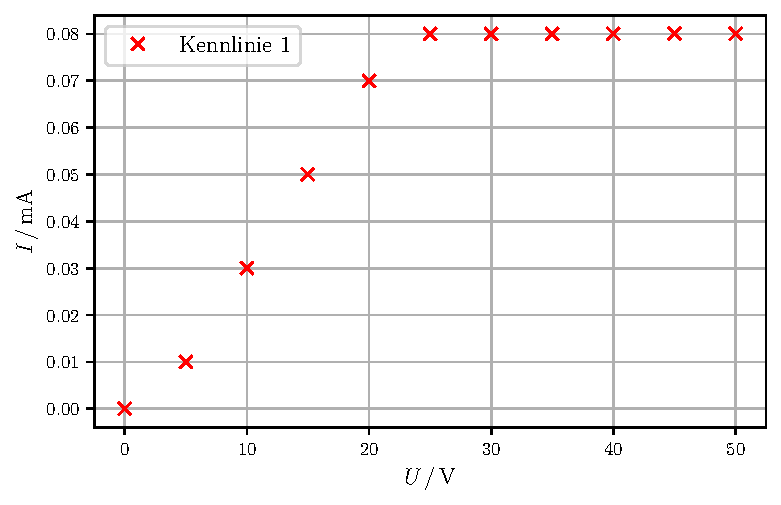
\includegraphics[width=\textwidth]{plot_k1.pdf}
  \caption{Kennlinie 1 mit $I_\text{Heiz} = \qty{1,9}{\ampere}$.}
  \label{fig:k1}
  \end{subfigure}\hfill
  \begin{subfigure}{0.49\columnwidth}
  \centering
  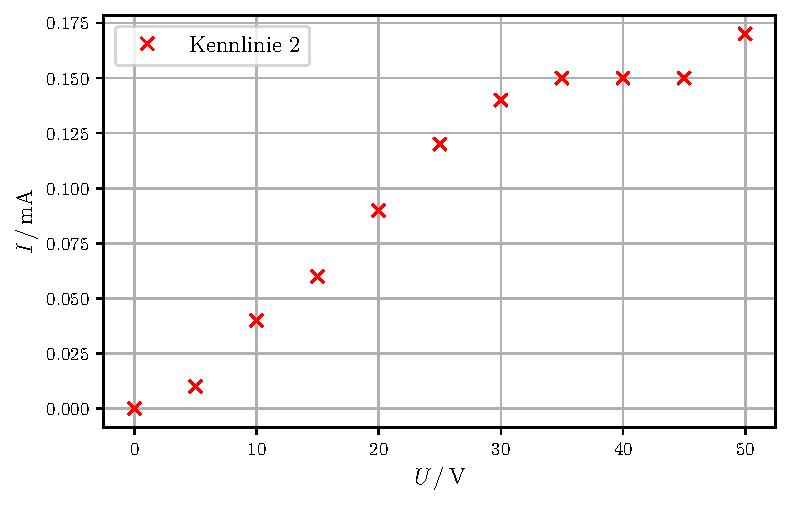
\includegraphics[width=\textwidth]{plot_k2.pdf}
  \caption{Kennlinie 2 mit $I_\text{Heiz} = \qty{2,0}{\ampere}$.}
  \label{fig:k2}
  \end{subfigure}
  
  \medskip
  
  \begin{subfigure}{0.49\columnwidth}
  \centering
  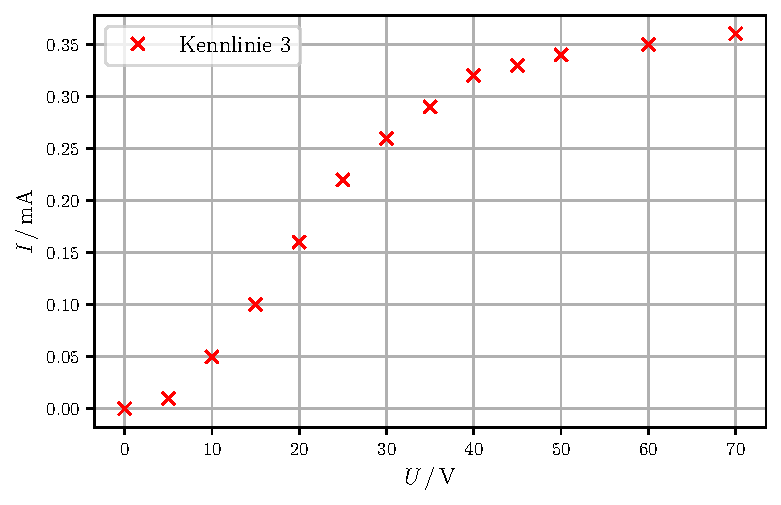
\includegraphics[width=\textwidth]{plot_k3.pdf}
  \caption{Kennlinie 3 mit $I_\text{Heiz} = \qty{2,1}{\ampere}$.}
  \label{fig:k3}
  \end{subfigure}\hfill
  \begin{subfigure}{0.49\columnwidth}
  \centering
  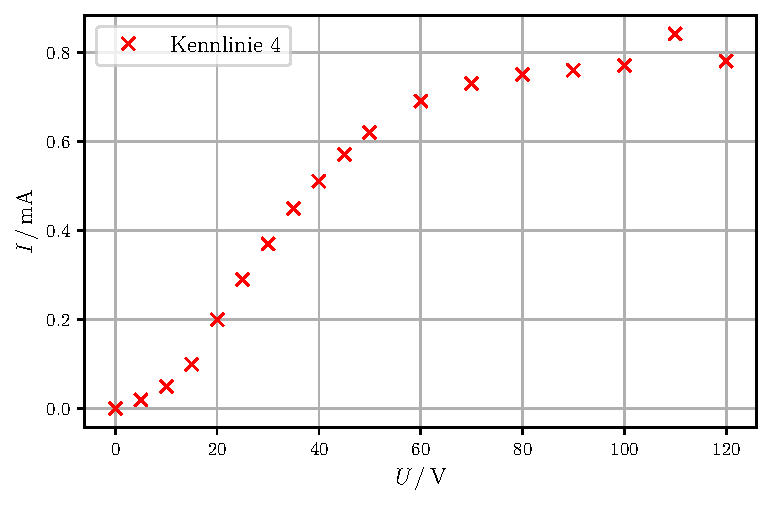
\includegraphics[width=\textwidth]{plot_k4.pdf}
  \caption{Kennlinie 4 mit $I_\text{Heiz} = \qty{2,2}{\ampere}$.}
  \label{fig:k4}
  \end{subfigure}
  
  \medskip
  
  \begin{subfigure}{0.7\columnwidth}
  \centering
  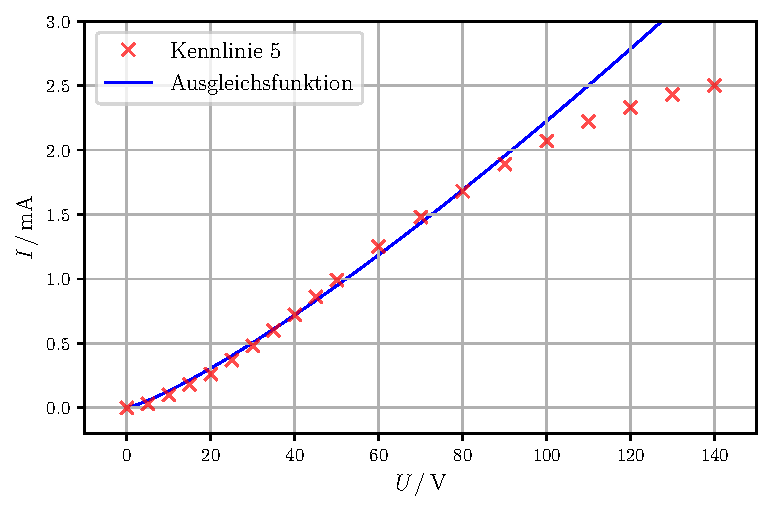
\includegraphics[width=\textwidth]{plot_k5.pdf}
  \caption{Kennlinie 5 mit $I_\text{Heiz} = \qty{2,4}{\ampere}$.}
  \label{fig:k5}
  \end{subfigure}

  \caption{Die fünf Kennlinien mit den jeweils angelegten Heiztrömen.}
  \label{fig:k}

\end{figure}

Der Sättigungstrom wird ab einer asymptotischen Entwicklung der Kennlinie abgelesen:
\begin{align*}
  \text{Kennlinie 1} : \quad I_\text{S} &= \qty{0,08}{\milli\ampere} \\
  \text{Kennlinie 2} : \quad I_\text{S} &= \qty{0,15}{\milli\ampere} \\
  \text{Kennlinie 3} : \quad I_\text{S} &= \qty{0,35}{\milli\ampere} \\
  \text{Kennlinie 4} : \quad I_\text{S} &= \qty{0,75}{\milli\ampere} \\
  \text{Kennlinie 5} : \quad I_\text{S} &= \qty{2,33}{\milli\ampere}
\end{align*}


\subsection{Raumladungsgesetz}

Mithilfe des Langmuir-Schottkyschen Raumladungsgesetzes nach \autoref{eq:lsr} wird bei Kennlinie 5 eine Ausgleichsrechung durchgeführt. 
Dabei werden der Faktor $\frac{1}{a^{2}}$ und der Exponent $b$ als freiee Parameter gewählt.
\begin{equation*}
  I= \frac{4}{9} \varepsilon_{0} \sqrt{\frac{2 e_{0}}{m_{0}}} \cdot \frac{U^{b}}{a^2}
\end{equation*}
Die dadurch bestimmten Parameter ergeben sich zu
\begin{align*}
  a &= (\num{-17.475(1.148)}) \cdot 10^{-3} \\
  b &= (\num{1.232(0.031)}) \, . 
\end{align*}
Die sich so ergebende Funktion wird in \autoref{fig:k5} eingezeichnet.


\subsection{Anlaufstromgebiet}

In \autoref{tab:anlaufstrom} sind die Messdaten des Anlaufstromgebietes eingetragen. Dabei wurde
eine Heizspannung von $I_{\text{Heiz}} = \qty{2.4}{\ampere}$ gewählt.
\begin{table}
  \centering
  \caption{Messwerte des Anlaufstroms.}
  \label{tab:anlaufstrom}
  \begin{tabular}{c c}
    \toprule
    $U \mathbin{/} \unit{\volt}$ &
    $I \mathbin{/} \unit{\nano\ampere}$ \\
    \midrule
    0,00 & 7,0000 \\
    0,10 & 8,1000 \\
    0,20 & 4,6500 \\
    0,30 & 2,5000 \\
    0,40 & 1,2000 \\
    0,50 & 0,4500 \\
    0,60 & 0,4000 \\
    0,70 & 0,2000 \\
    0,80 & 0,0600 \\
    0,90 & 0,0230 \\
    0,96 & 0,0005 \\
    \bottomrule
  \end{tabular}
\end{table}

Mithilfe dieser Messdaten wird eine Ausgleichsrechung nach \autoref{eq:anlaufstromgebiet}
\begin{equation}
  I=a \cdot \exp \left(\frac{-e_{0} U}{k_{\text{B}} \cdot b}\right)
\end{equation}
durchgeführt und in \autoref{fig:anlaufstrom}. Die Parameter ergeben sich dabei zu
\begin{align*}
  a &= \qty{13.228(0.240)}{\nano\ampere} \, , \\
  b &= \qty{2131(70)}{\kelvin} \, . 
\end{align*}
Dabei entspricht der Parameter $b$ der gesuchten Temperatur $T = \qty{2131(70)}{\kelvin}$ .

\begin{figure}[H]
  \centering
  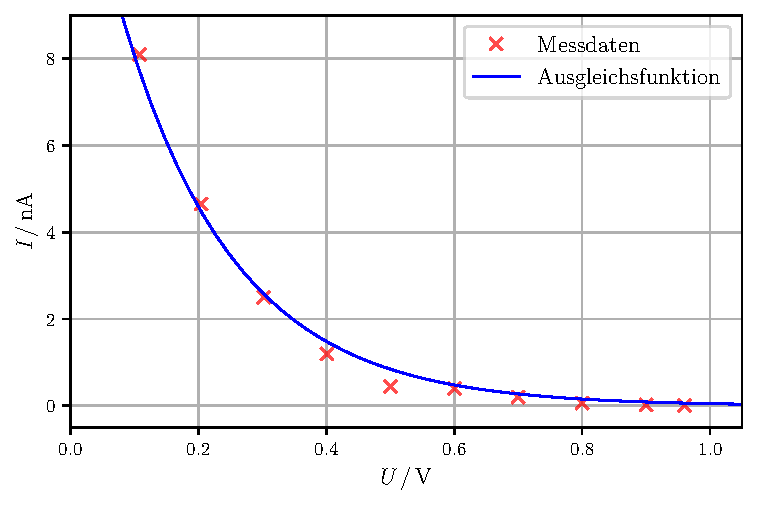
\includegraphics[width=0.8\textwidth]{plot6.pdf}
  \caption{Das Anlaufstromgebiet bei einem Heizstrom von $I_\text{Heiz} = \qty{2,5}{\ampere}$.}
  \label{fig:anlaufstrom}
\end{figure}


\subsection{Kathodentemperatur}

Die Kathodentemperatur $T$ lässt sich aus einer Betrachtung der Leistungsbilanz bestimmen.
Die zugeführte Leistung beträgt
\begin{equation*}
  N_{\text{zu}}=U_{\text{Heiz}} I_{\text{Heiz}} \, ,
\end{equation*}
Diese wird über Wärmestrahlung und Wärmeleitung abgegeben. 
Die Wärmeleitung der Fadenhalterung wird durch $N_{\text{WL}} = \qty{1}{\watt}$ abgeschätzt. 

Die Srahlungsleistung ergibt sich nach dem Stefan-Boltzmannschen Gesetz zu
\begin{equation*}
  N_{\mathrm{W}}=f \eta \sigma T^{4} \, .
\end{equation*}

Mit den Größen:
\begin{align*}
  & \text{Kathodenoberfläche} & \quad & f = \qty{0.32}{\centi\meter\squared} \\
  & \text{Emissionsgrad der Oberfläche} & \quad & \eta=0,28 \\
  & \text{Stefan-Boltzmannsche Strahlungskonstante} & \quad & \sigma = \qty{5.7e-12}{\watt\per\square\centi\meter\kelvin\tothe{-4}} 
\end{align*}

Aus dem Energiesatz folgt insgesamt
\begin{align*}
N_{\text{zu}} &=N_{\text{W}}+N_{\text{WL}} \\
\Leftrightarrow \quad U_{\text{Heiz}} I_{\text{Heiz}} &=f \eta \sigma T^{4}+N_{\text{WL}}
\end{align*}
Mit der daraus nach $T$ umgeformten Gleichung
\begin{align*}
  T &= \sqrt[4]{ \frac {U_\text{Heiz} I_\text{Heiz} - N_\mathrm{WL}} {f \eta \sigma} } 
\end{align*}
ergeben sich die in \autoref{tab:temp} dargestellten Werte für die Kathodentemperaturen.
\begin{table}
  \centering
  \caption{Berechnete Temperaturen der Kathoden zu den verschiedenen Heiztrömen und -spannungen.}
  \label{tab:temp}
  \begin{tabular}{c c c}
    \toprule
    $U_\text{Heiz} \mathbin{/} \unit{\volt}$ &
    $I_\text{Heiz} \mathbin{/} \unit{\ampere}$ &
    $T \mathbin{/} \unit{\kelvin}$ \\
    \midrule
    4,5 &  1,9 & 1960,83 \\
    4,9 &  2,0 & 2037,39 \\
    5,0 &  2,1 & 2076,75 \\
    5,5 &  2,2 & 2159,16 \\
    6,2 &  2,4 & 2283,24 \\
    \bottomrule
  \end{tabular}
\end{table}


\subsection{Austrittsarbeit des Kathodenmaterials}

Zur Berechnung der Austrittsarbeit der Elektronen wird die Richardson-Gleichung \ref{eq:Richardson} nach
$e_{0} \Phi$ umgestellt
\begin{equation*}
  W_{\text{A}} = e_{0} \Phi = -T k_{\text{B}} \ln \left(\frac{j_{\text{S}} h^{3}}{4 \pi e_{0} m_{0} k_{\text{B}}^{2} T^{2}}\right)
  \quad \text{mit} \quad
  j_\text{S} = \frac{I_\text{S}}{f}
\end{equation*}
als Sättigungsstromdichte, die durch den Sättigungsstrom durch die Kathodenoberfläche ausgedrückt werden kann.

Die sich somit ergebende Austrittsarbeit von Wolfram wird in \autoref{tab:arbeit} angegeben.
\begin{table}
  \centering
  \caption{Berechnete Austrittsarbeiten für Wolfram.}
  \label{tab:arbeit}
  \begin{tabular}{c c c}
    \toprule
                &  $W_{\text{A}} \mathbin{/} \mathrm{eV}$ &
                   $W_{\text{A}} \mathbin{/} \mathrm{J} \cdot 10^{-19}$ \\
    \midrule
    Kennlinie 1 &  3,148 & 5,043 \\
    Kennlinie 2 &  3,142 & 5,034 \\
    Kennlinie 3 &  3,066 & 4,913 \\
    Kennlinie 4 &  3,074 & 4,925 \\
    Kennlinie 5 &  3,162 & 5,066 \\
    \bottomrule
    \end{tabular}
\end{table}

Damit ergibt sich für den Mittelwert und die Varianz der fünf Austrittsarbeiten zu
\begin{equation*}
  \overline{W_{\text{A}}} = \qty{3.12(4)}{\eV} \, .
\end{equation*}
